\documentclass[t]{beamer}
\usepackage[orientation=landscape,size=custom,width=115,height=100,scale=1]{beamerposter}
\usepackage{textpos}
%\usepackage[absolute,overlay]{textpos} ??
\usepackage[absolute]{textpos}
\usepackage{tikz}
\usepackage{url}
\usepackage{fancybox}
\usepackage{tcolorbox}
\usepackage{verbatim}
\usepackage{multirow}
\usepackage{booktabs}
\usepackage{graphicx}
\usepackage{caption}
\usepackage{lmodern} % Font style
\usepackage{ragged2e} % For using \justify

\setbeamerfont{frametitle}{size=\Huge,series=\bfseries}
\setbeamerfont{framesubtitle}{size=\huge}
\setbeamerfont{block title}{size=\large,series=\bfseries}
\setbeamerfont{block body}{size=\normalsize}
\setbeamerfont{caption}{size=\small}

\addtobeamertemplate{frametitle}{\vspace*{5cm}}{\vspace*{5cm}}
\addtobeamertemplate{block begin}{\vspace*{40pt}}{}

\setbeamertemplate{frametitle}[default][center]
\setbeamertemplate{caption}[numbered]
\setbeamertemplate{itemize items}{$\circ$}

\definecolor{arsenic}{rgb}{0.23, 0.27, 0.29}
\definecolor{mycyan}{rgb}{0.0, 0.55, 0.55}
\definecolor{mygray}{rgb}{0.23, 0.27, 0.29}
\definecolor{myblue}{rgb}{0.16, 0.32, 0.75}
\definecolor{mygreen}{rgb}{0.05, 0.5, 0.06}
\definecolor{mypurple}{rgb}{0.45, 0.31, 0.59}
\definecolor{myred}{rgb}{0.82, 0.1, 0.26}

\setbeamercolor{background canvas}{bg=arsenic}
\setbeamercolor{frametitle}{fg=white}
\setbeamercolor{framesubtitle}{fg=white}
\setbeamercolor{textblock}{fg=white,bg=white}
\setbeamercolor{normal text}{fg=black}
\setbeamercolor{block body}{bg=white, fg=black}

\setbeamersize{text margin left=3cm,text margin right=3cm}

% Different colors for lightcurve plot, increase font size too
% Print copies of poster?
% Print abstract?
% Linkedin, my info, resume, etc.
% Add twitter, facebook, github, whatev. to poster itself

\begin{document}

\begin{frame}[t]
    \frametitle{An Overview of Coronal Seismology and Application to Data
        from AIA/SDO}
    \framesubtitle{Laurel Farris*, R. T. James McAteer*}
    \begin{center}
        \textcolor{white}{\normalsize New Mexico State University}
    \end{center}
    \begin{block}{}
    \begin{columns}
        \column{0.35\textwidth}
        \setbeamercolor{block title}{fg=myblue}
        \setbeamercolor{description item}{fg=myblue}
        \setbeamercolor{enumerate item}{fg=myblue}
        \setbeamercolor{caption name}{fg=myblue}
        \begin{block}{Introduction \& motivation}
            The method of coronal seismology involves the observation and
            characterization of disturbances in the solar corona. Such disturbances
            can be in the form of standing oscillations in coronal structures or
            waves propagating across the surface and through the atmosphere
            between the photosphere and corona.
            These disturbances can be triggered by a variety of phenomena,
            such as the continuous motions of the photosphere around the footpoints
            of coronal loops, or the impulsive burst of motion from a flare or
            coronal mass ejection (CME). The characteristics of the waves produced
            by this activity can reveal information about the flares/CMEs themselves.
            Coronal seismology also offers a way to extract coronal parameters that
            are difficult to observe directly, such as magnetic field strength.
        \end{block}

        \begin{block}{Magnetohydrodynamics (MHD)}
            \begin{columns}
                \column{0.50\textwidth}
                \begin{figure}
                    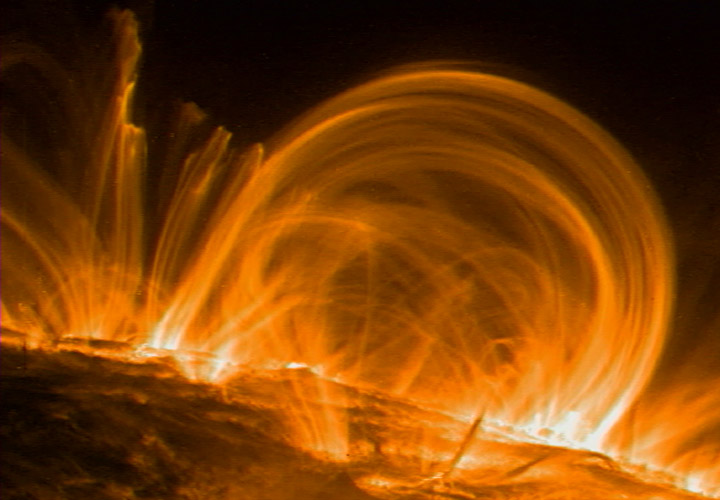
\includegraphics[width=0.9\textwidth]{../loop.jpg}
                    \caption{A typical coronal loop}
                \end{figure}
                \begin{figure}
                    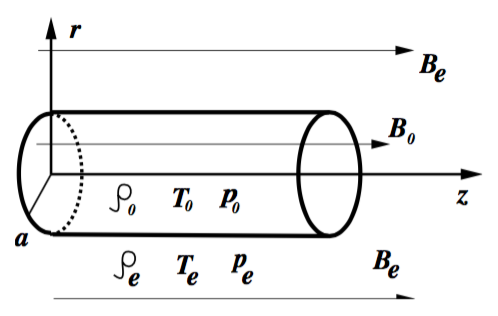
\includegraphics[width=0.9\textwidth]{../cylinder.png}
                    \caption{Cylindrical model of a waveguide}
                \end{figure}
                \column{0.45\textwidth}
                \par\vspace{20pt}
                Coronal seismology is based on the theories of
                ideal magnetohydrodynamics (MHD), where
                waves and oscillations in the corona are modelled as propagating
                in a uniform magnetic field, guided by a straight cylindrical
                flux tube (\textcolor{myblue}{figure 2}).
                Coronal loops, such as the one pictured in
                \textcolor{myblue}{figure 1}, can act as
                a waveguide, and
                are just one of the structures in the corona
                that support MHD modes. These modes are
                Characterized by different wave speeds that are determined by
                the gas density ($\rho$), gas temperature ($T$),
                gas pressure ($P$), and magnetic field strength
                ($\vec{B}$), both interior and exterior to the waveguide
                (see figure 2 at left). Two of the more familiar characteristic
                speeds are:
                \vspace{20pt}
                \begin{description}
                    \item [\textbf{Sound speed}]
                        $C_s\propto\sqrt{\cfrac{P}{\rho}}\propto\sqrt{T}$
                    \par\vspace{20pt}
                    \item [\textbf{Alfv\'en speed}]
                        $V_A\propto\cfrac{B}{\sqrt{\rho}}$
                \end{description}
                \vspace{20pt}
                Other structures that can support MHD modes include sunspot pores
                and magnetic bright points. A bright point in a coronal hole is
                analyzed for this project (see \textcolor{mygreen}{Data} and
                subsequent sections).
            \end{columns}
        \end{block}

        \begin{block}{Coronal Seismology}
            \begin{columns}
                \column{0.45\textwidth}
                \begin{figure}
                    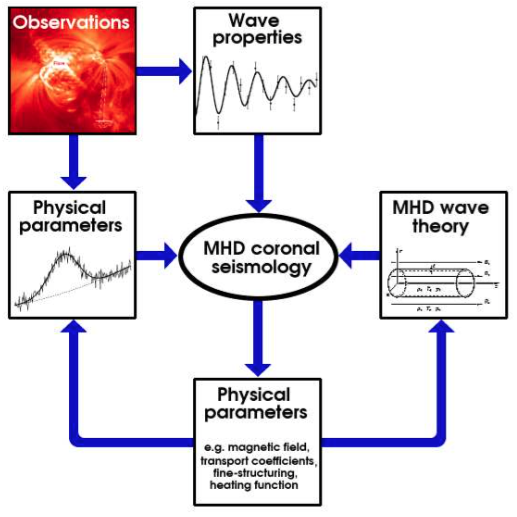
\includegraphics[width=0.9\textwidth]{../schematic.png}
                    \caption{Schemetic of how physical properties and
                        wave properties are connected by coronal seismology.
                    }
                \end{figure}
                \column{0.45\textwidth}
                The method of coronal seismology can be summarized in four
                steps:
                \begin{enumerate}
                    \item Observe disturbances
                    \item Measure physical parameters
                    \item Identify wave properties
                    \item Extract physical parameters
                \end{enumerate}
                How these disturbances are observed depends on a number of
                factors: direction of travel relative to the line-of-sight,
                whether or not they show visible variations (such as intensity
                changes, which correspond to density changes in the plasma),
                and whether the spatial variations occur on sizescales for
                which sufficient resolution is available.
                \textcolor{myblue}{Figure 3} shows how direct observations of
                physical properties and extracted properties are interrelated
                throught coronal seismology.
            \end{columns}
        \end{block}

        \begin{block}{MHD wave modes}
            \begin{columns}
                \column{0.45\textwidth}
                \begin{figure}
                    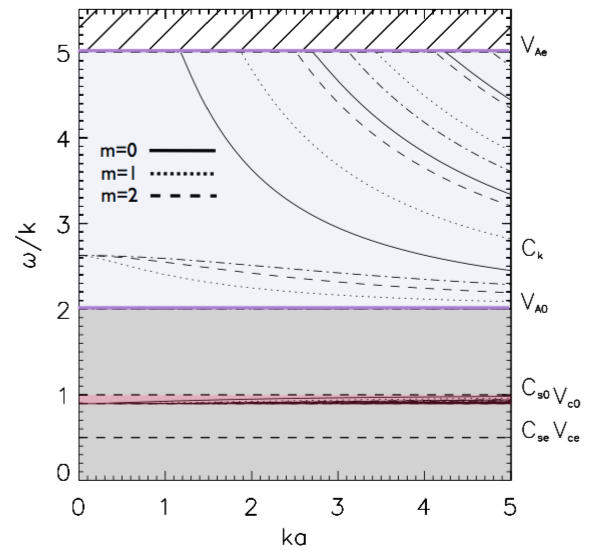
\includegraphics[width=0.9\textwidth]{../disp_diagram.png}
                    \caption{Dispersion diagram for MHD modes}
                \end{figure}
                \column{0.55\textwidth}
                \textcolor{myblue}{Figure 4} shows the phase velocities ($\omega/k$), expressed as
                multiples of the internal sound speed ($C_0$) of the waveguide,
                as functions of wavenumber ($ka$) for different types
                of MHD modes.
                In general, MHD modes are categorized as follows:
                \par\vspace{5pt}
                \begin{description}
                    \item [\textbf{Magnetoacoustic}] Analagous to regular acoustic
                        waves, (or sound waves), these are pressure-driven
                        waves in the presence of a magnetic field.
                        They are sub-divided into two more groups:
                        \begin{description}
                            \item [\textbf{Fast}] Phase speeds faster than the
                                internal Alfv\'en speed ($V_{A0}$).
                            \item [\textbf{Slow}] Phase speeds close to the
                                internal sound speed ($C_{0}$).
                        \end{description}
                    \par\vspace{10pt}
                    \item [\textbf{Alfv\'en}] These are magnetically driven waves,
                        with speeds determined by $\vec{B}$.
                \end{description}
            \end{columns}
        \end{block}

        \column{0.2\textwidth}

        \setbeamercolor{block title}{fg=mygreen}
        \setbeamercolor{description item}{fg=mygreen}
        \setbeamercolor{enumerate item}{fg=mygreen}
        \setbeamercolor{caption name}{fg=mygreen}
        \begin{block}{Data}
            Some of the techniques of coronal seismology were tested on a
            series of images from the
            Atmospheric Imaging Assembly (AIA) instrument
            on board the \emph{Solar Dynamics Observatory (SDO)},
            at the 193 \AA{} line (Fe XII and Fe XXIV). This line occurs at
            temperatures of around 10$^{6}$ K.
            The data set spanned one hour in July of 2012 and were taken
            at a cadence of 12 seconds, for a total of 300 images.
            The first image in the series is shown in
            \textcolor{mygreen}{figure 5}.
            \par\vspace{10pt}
            \begin{figure}
                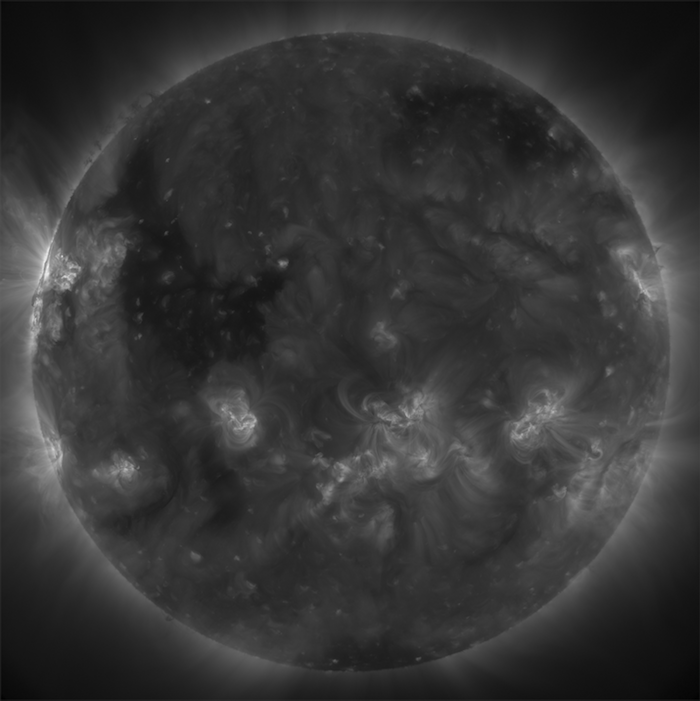
\includegraphics[width=0.7\textwidth]{full_disk.png}
                \caption{First image in the time-series from
                    AIA/\emph{SDO}
            }
            \end{figure}
            The full disk shows an active region in the lower right, a coronal hole
            in the upper left, and some quiet sun areas in the upper right.
            A bright point from the coronal hole was selected for analysis,
            and is shown in \textcolor{mygreen}{figure 6}.
            \par\vspace{20pt}
            \begin{figure}
                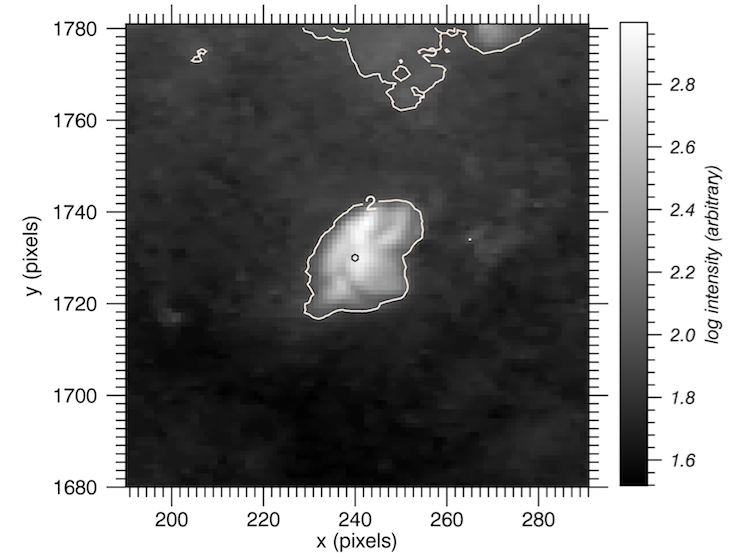
\includegraphics[width=\textwidth]{../bp1_contour.png}
                \caption{Image of the single bright point analyzed for
                    this project.}
            \end{figure}
            The contours around the bright point
            outline its estimated physical boundary,
            which was determined using an intensity cutoff.
            The areas in the upper region of the image were also
            above this intensity threshold,
            and therefore are also outlined. The circle in the center indicates
            the location of the pixel that was correlated with every
            other pixel in the image (see \textcolor{mycyan}{Analysis techniques}).
        \end{block}

        \setbeamercolor{block title}{fg=mycyan}
        \setbeamercolor{description item}{fg=mycyan}
        \setbeamercolor{enumerate item}{fg=mycyan}
        \setbeamercolor{caption name}{fg=mycyan}
        \begin{block}{Analysis techniques}
            Two general analysis techniques were applied to this data set:
            \begin{description}
                \item [\textbf{Lightcurves}] The variation in intensity of the bright
                    point, along with the size as determined by the intensity
                    threshold, are both plotted in \textcolor{myred}{figure 7}
                    as functions of time. The phase difference between intensity and
                    size can be an indication of the type of MHD mode (for instance, the
                    so-called ``sausage modes'' have a characteristic phase
                    difference equal to $\pi$ between the two).
                \item [\textbf{Cross-correlation}] To search for patterns in the
                    horizontal direction (i.e.\ across the surface at the
                    same height), a cross-correlation was calculated between
                    the central pixel in the bright point and every other
                    pixel in figure 6 across the time-series.
                    With this technique, the distance, speed,
                    and/or oscillation period of a disturbance traveling
                    outward from the brightpoint could be potentially be extracted.
            \end{description}
        \end{block}

        \column{0.3\textwidth}
        \setbeamercolor{block title}{fg=myred}
        \setbeamercolor{description item}{fg=myred}
        \setbeamercolor{enumerate item}{fg=myred}
        \setbeamercolor{caption name}{fg=myred}

        \begin{block}{Lightcurve results}
            \begin{columns}
                \column{0.6\textwidth}
                \begin{figure}
                    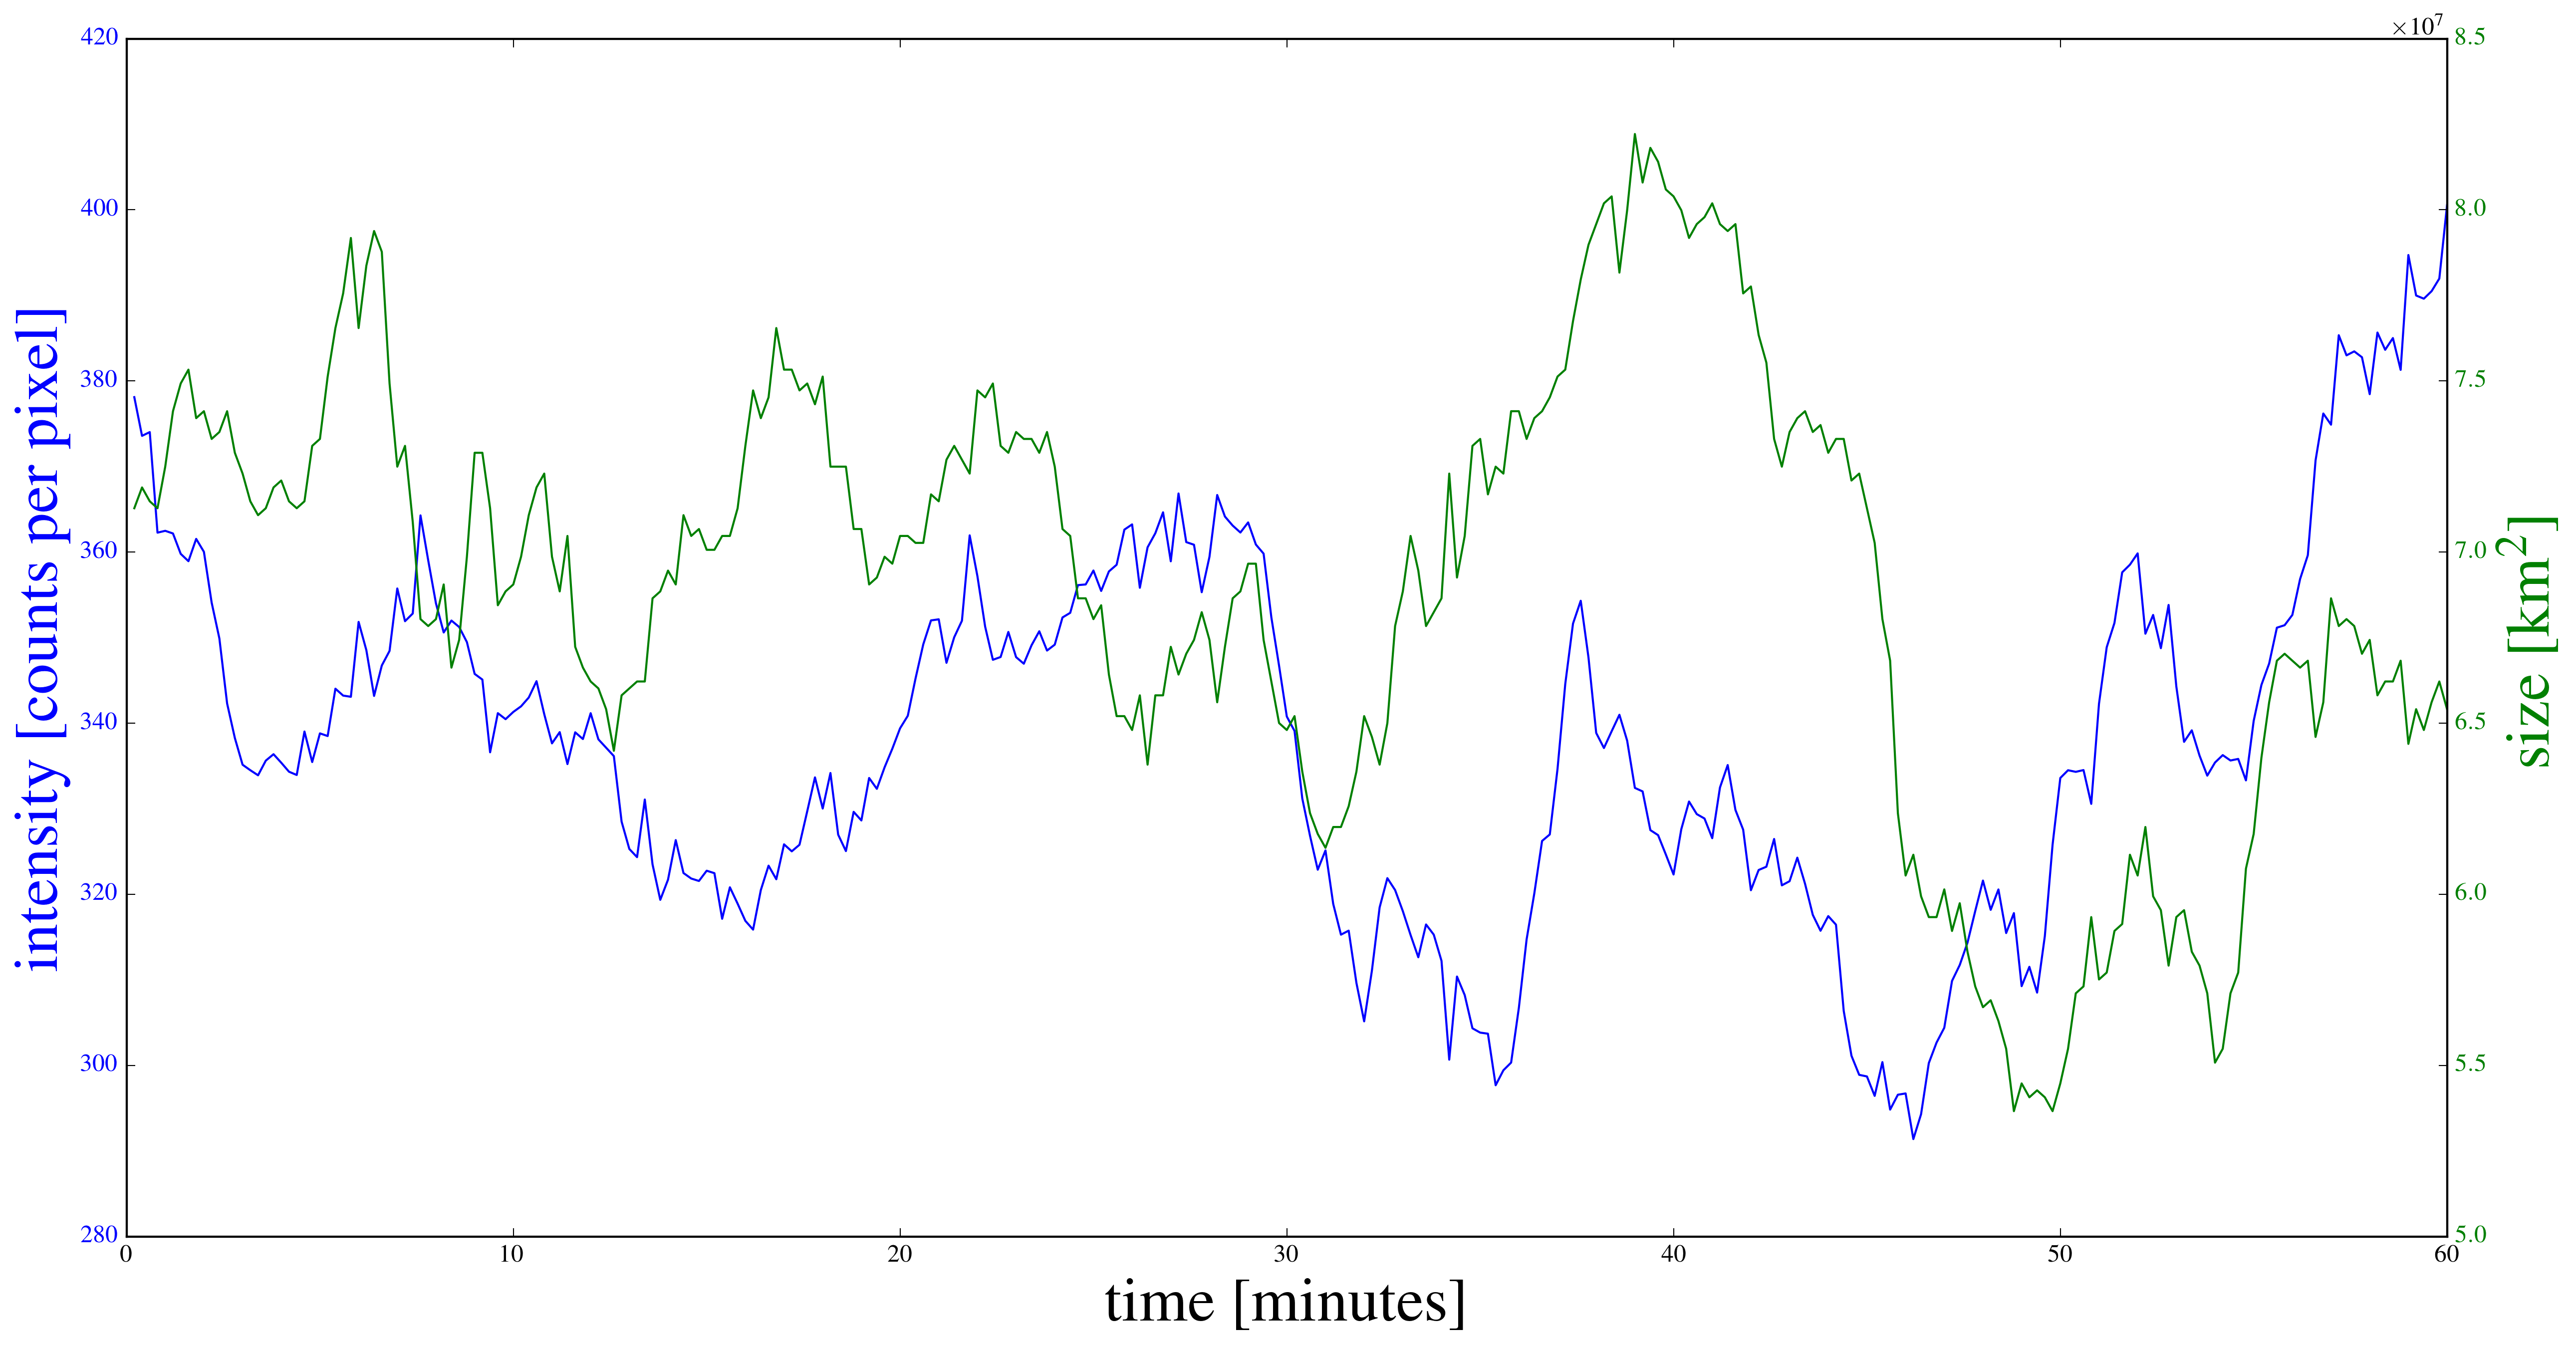
\includegraphics[width=\textwidth]{../plot2.png}
                    \caption{Size and intensity of the
                        bright point as functions of time throughout the entire
                        data series.}
                \end{figure}
                \column{0.3\textwidth}
                \vspace*{\fill}
                \clearpage
                \textcolor{myred}{Figure 7} shows how the size and intensity
                (per unit area) varied over the course of one hour.
                There appears to be a similar pattern between the two;
                they become closer in phase at the end of the time series.
                Further numerical analysis, such as a fourier transform,
                is needed to extract periodicities and draw more
                conclusive results.
                \vfill
                \clearpage
            \end{columns}
        \end{block}

        \begin{block}{Cross-correlation results}
            \begin{figure}
                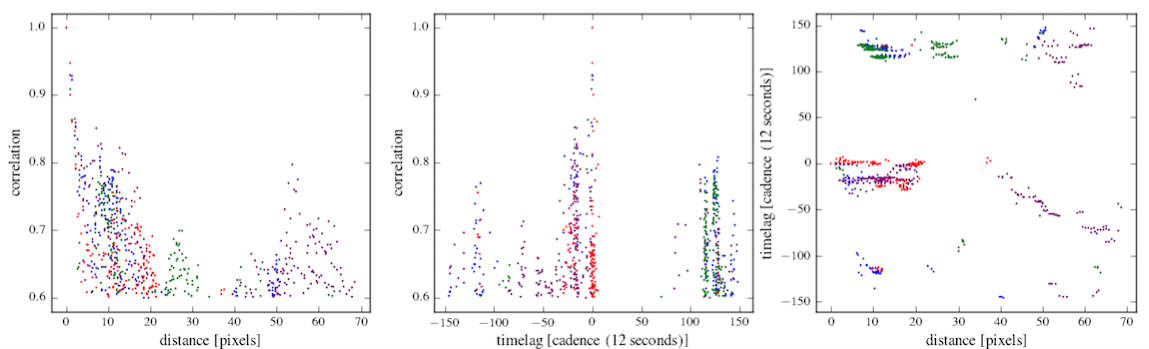
\includegraphics[width=\textwidth]{../test2.png}
                \caption{Relationship between the cross-correlation,
                timelag, and radial distance from central pixel.}
            \end{figure}
            \begin{columns}
                \column{0.4\textwidth}
                \begin{figure}
                    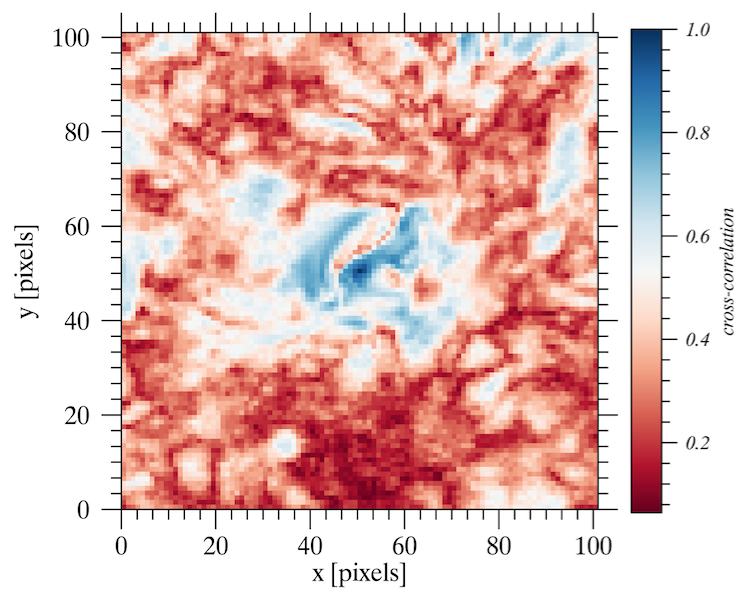
\includegraphics[width=\textwidth]{cc_color_2.png}
                    \caption{Image illustrating the maximum correlation
                        value of each pixel with the central pixel.}
                \end{figure}
                \column{0.4\textwidth}
                \begin{figure}
                    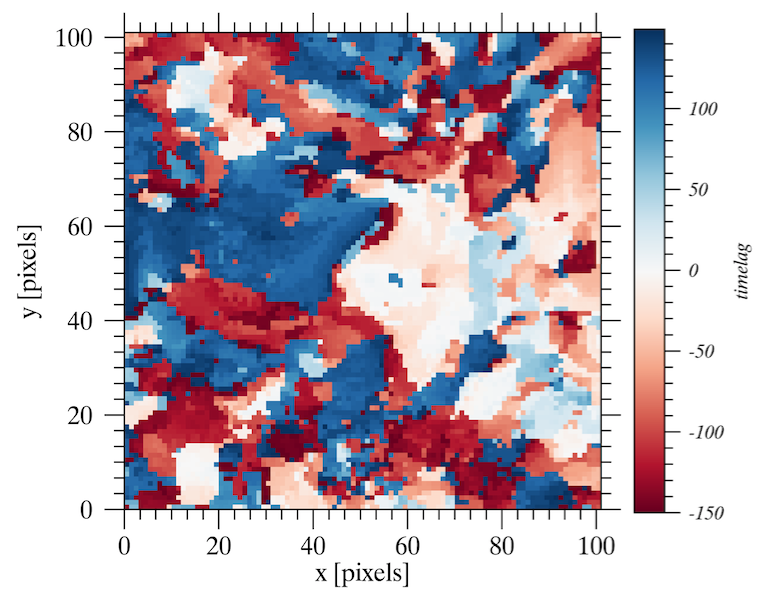
\includegraphics[width=\textwidth]{tt_color_2.png}
                    \caption{Image of the timelag corresponding to each
                    correlation value in \textcolor{myred}{figure 9}.}
                \end{figure}
            \end{columns}
            \par\vspace{30pt}
            After running the cross-correlation, the highest values were
            plotted as functions of both timelag and distance. Additionally,
            the timelag was plotted as a function of distance. All three plots
            are shown in \textcolor{myred}{figure 8}.
            The value of the maximum correlation value of each pixel with
            the central pixel is illustrated as an image in
            \textcolor{myred}{figure 9}.
            The corresponding timelag at which each of these correlation
            values occurred is similarly illustrated in
            \textcolor{myred}{figure 10}.
            %\par\vspace{250pt}
        \end{block}
        \begin{columns}
            \column{0.5\textwidth}
            \setbeamercolor{block title}{fg=mypurple}
            \begin{block}{Conclusions \& Future Work}
                Some additional calculations are required for more conclusive
                results: a fourier transform on
                the plots in \textcolor{myred}{figure 7} is needed to
                extract potential periodic information.
                Data from the Helioseismic and Magnetic Imager (HMI)
                on \emph{SDO} during the
                same time as the data used here could reveal information about
                the magnetic counterpart to the bright point in the photosphere.
                There are many bright points in the coronal hole, along with
                quiet sun areas and active regions to look at as well.
            \end{block}
            \column{0.5\textwidth}
            \setbeamercolor{block title}{fg=mygray}
            \begin{block}{Acknowledgements}
                Thanks to my advisor, Dr.\ James McAteer for guidance throughout
                this project.
            \end{block}
            \begin{block}{References}
                Figure 1 is from \textcolor{myblue}{http://scied.ucar.edu/sun-coronal-loops}.
                Figures 2, 3, and 4 are from Nakariakov \& Verwichte (2005).
            \end{block}
        \end{columns}
        \par\vspace{3cm}
        
\includegraphics{nmsu.png}
    \end{columns}
\end{block}
\end{frame}

\end{document}
